\section{Implementaci\'on}
En esta secci\'on discutiremos las particularidades de cómo se llev\'o a cabo la implementaci\'on del m\'etodo propuesto en \cite{Felzenszwalb2004}. Lo primero a mencionar es que para segmentar una imagen el primer proceso es obtener una versi\'on en escala de grises de esta donde ademas se le aplica un filtro Gaussiano con parametro $\sigma=0.8$. Esto último se hace con el fin de disminuir el ruido de \textit{artifacts} que pueden llegar a estar presentes en la imagen digital. \\
\indent Como se mencion\'o en la secci\'on anterior el algoritmo requiere intrinsecamente dos funcionalidades:
\begin{itemize}
	\item Ordenar las aristas de forma no decreciente.
	\item Poder determinar si dos vértices pertenecen a la misma componente y en caso de ser necesario juntarlas.
\end{itemize}

\indent Como estas dos partes no influyen sobre la otra las analizaremos por separado y tendremos como definici\'on general que $\#V(G)=n=$``Cantidad de píxeles en la imagen''.

\subsection{Ordenamiento de las aristas}
Lo primero que hay que definir es qué conjunto de aristas se toman, ya que la definici\'on del conjunto $E$ en la secci\'on anterior admite tomar cualquier subconjunto de aristas posibles. En lo desarrollado en \cite{Felzenszwalb2004} (y en este trabajo) se considera que $(v_i,\ v_j)\in E$ si y solo si $v_j$ est\'a entre los 8 píxeles m\'as cercanos de $v_i$, as\'i $\#E=m<8n=\mathcal{O}(n)$. \\
\indent Adem\'as se utiliz\'o como estructura de representaci\'on de grafos una \textit{lista de aristas}: guardando en una lista doblemente enlazada las aristas en forma de triplas (peso, cola, cabeza) y el valor $n$ de la cantidad de vértices totales. Luego se plantea el siguiente procedimiento para obtener el grafo $G$ de la imagen a segmentar:

\begin{algorithm}
\caption{Imagen a lista de aristas ordenadas por peso}
\label{img2sorted}
\begin{algorithmic}[1]
\Procedure{img2sortedGraph}{$Img$}
\State $G$ $\gets$ nuevoGrafo($\{\}$, Img.height * Img.width)
\State $aristas$ $\gets$ vector(lista(arista)) (256, $\{\}$)
\State Para $pix$ en $Img$:
\State \indent 	Para $vec$ en 8masCercanos($pix$), si $(vec,pix)\notin E$:
\State \indent	\indent 	$nueva\_arista$ $\gets$ ($pix-vec$, pix, vec)
\State 			insertar $nueva\_arista$ en la lista de $aristas$[pix-vec]
\State $G.aristas$ $\gets$ juntarListasEnOrden($aristas$) 
\EndProcedure
\end{algorithmic}
\end{algorithm}

\indent Este procedimiento genera las aristas seg\'un el criterio planteado y las guarda de forma ordenada con una complejidad $\mathcal{O}(n)$. \\
\indent Respecto a la correctitud generamos las aristas sin repetirlas y las guardamos en el vector $aristas$ en función de su peso. Luego encadenando las listas de la posici\'on $0$ a la $255$ del vector obteniendo una \'unica lista en donde los pesos se encuentrar ordenados de manera no decreciente. En esencia: se implement\'o como un \textit{counting sort}. \\
Para deducir la complejidad podemos ver que las l\'ineas $1$ y $2$ toman tiempo constante, luego el ciclo principal revisa una cantidad de $8n$ píxeles y sobre ellos realiza operaciones de tiempo constante. Por último encadenar las listas en la l\'inea $8$ consiste en reencadenar $256$ punteros, tomando tiempo constante para cada uno de ellos. Por lo tanto la complejidad del procedimiento resulta $\mathcal{O}(n)$. 

\subsection{Representaci\'on de componentes}
En el algoritmo propuesto en la secci\'on de desarrollo se vi\'o que era necesario poder mantener en simultáneo para cada píxel a qué componente pertenec\'ia, saber el tama\~no de una componente y eventualmente unir dos componentes. Notar que como se mencion\'o previamente la segmentaci\'on es una partici\'on de $V$ y por lo tanto cada píxel pertenece a un solo conjunto dentro de la partici\'on. A raíz de esto se puede modelar este problema como mantener la partici\'on en conjuntos disjuntos entre sí. A esta estructura se la llama \textit{Disjoint set} y provee la siguiente interfaz:
\begin{itemize}	
	\item crear(n): crea $n$ conjuntos disjuntos.
	\item find(i): devuelve el identificador del conjunto al que pertenece el elemento $i$.
	\item unite(i,j): junta los conjuntos a los que pertenecen $i$ y $j$ .
	\item tam(i): devuelve el cardinal del conjunto al que pertenece el elemento $i$.
\end{itemize}

A continuaci\'on discutiremos las posibles implementaciones de este tipo de datos. Todas las implementaciones tienen en com\'un que se utiliza un arreglo $tams$ en su representaci\'on interna tal que $tams[i]=$``tama\~no del conjunto identificable por $i$'' para $i$ un identificador de conjunto. Además todas las implementaciones utilizan la heurística de \textit{union by rank} que consiste en unir el conjunto de menor cardinal al de mayor cardinal al ejecutar el m\'etodo \textit{unite}.

\subsubsection{Arreglo de representaci\'on}
La estructura interna que utiliza es de un arreglo de $n$ posiciones donde $arr[i]=Id_i$ con $Id_i$ el identificador del conjunto al que pertenece el elemento $i$. Con esta representaci\'on la interfaz se implementa de la siguiente manera:
\begin{itemize}
	\item crear(n): inicializar un arreglo $arr$ de $n$ posiciones tal que $arr[i]=i$ $\rightarrow \mathcal{O}(n)$.
	\item find(i): devolver $arr[i] \; \rightarrow \mathcal{O}(1)$.
	\item unite(i,j): para toda posici\'on $k$ que cumple $arr[k]=Id_i$ cambiar por $arr[k]=j$, actualizar $tams[Id_j]+=tams[Id_i]$ $\rightarrow \Theta(n)$.
\end{itemize}

\subsubsection{Árbol de representantes}
De forma parecida a la estructura anterior se utiliza un arreglo de $n$ posiciones pero con la diferencia que $arr[i]$ ahora representa una \textit{relaci\'on de padre}. Esto nos define un árbol para cada conjunto y de esta forma podemos identificar al conjunto por la \textit{raíz} del arbol.

\begin{itemize}
	\item crear(n): inicializar un arreglo $arr$ de $n$ posiciones tal que $arr[i]=i$ $\rightarrow \mathcal{O}(n)$.
	\item find(i): Si $find[i]\neq i$: devolver $find[arr[i]]$ sino devolver $i$ $\rightarrow \mathcal{O}(n)$.
	\item unite(i,j): Obtener los representantes de $i$ y de $j$, $arr[Id_i]=Id_j$, actualizar $tams[Id_j]+=tams[Id_i]$ $\rightarrow \mathcal{O}(n)$.
\end{itemize}

\indent Notar que en peor caso esta estructura es te\'oricamente menos eficiente, ya que ahora obtener el identificador de un conjunto puede costar a lo sumo $n$ pasos.

\subsubsection{Árbol de representantes con \textit{path relinking}}
Su estructura interna es igual a la del \textit{arbol de representantes}, pero realiza la operaci\'on de \textit{find} con una diferencia: al buscar el identificador en la estructura anterior era necesario ``subir'' por la cadena de padres de un elemento para encontrar la raíz. A su vez esta raíz también es el identificador de todos los padres por los que se pas\'o para responder la query de \textit{find}, por lo tanto técnicamente al buscar al identificador de un elemento efectivamente se está resolviendo la query de buscar el identificador para toda la cadena de padres. Por lo tanto podemos aprovechar esto para cambiar el padre de todos estos elementos directamente por la raíz.\\

\begin{figure}[H]
\begin{center}
	\subfigure[Arbol de representantes G]{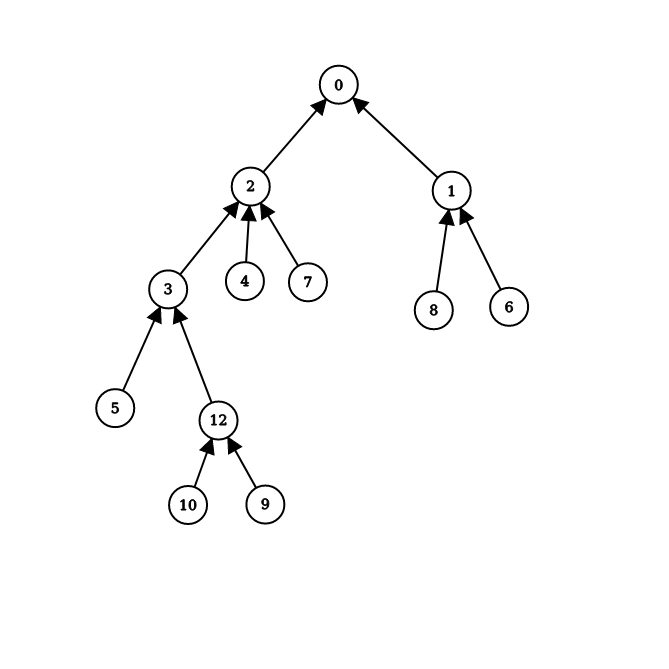
\includegraphics[scale=0.3]{plots/G.png}}
	\subfigure[G.$find(9)$]{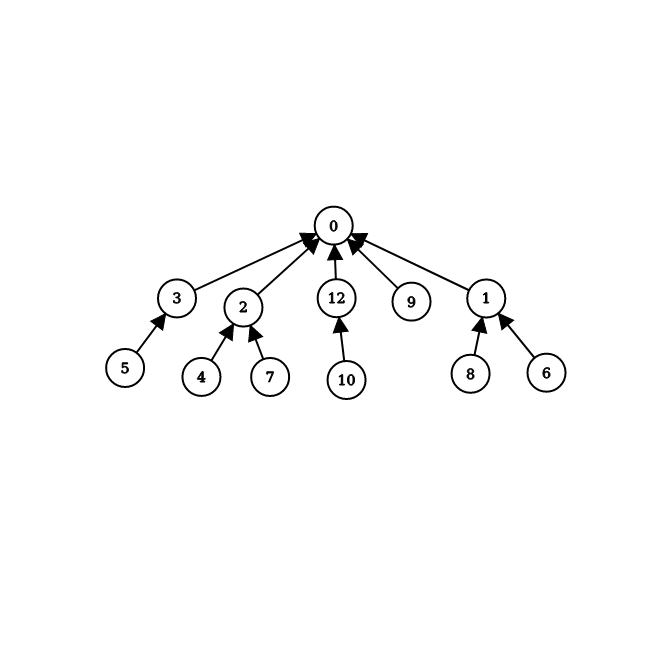
\includegraphics[scale=0.3]{plots/G_find9.png}}
\end{center}
\end{figure}

\vspace{-10mm}
Con esta representaci\'on Tarjan \cite{Tarjan} prob\'o que la operaci\'on \textit{find} (y por lo tanto \textit{unite}) toman tiempo $\mathcal{O}(\alpha(n))$ amortizado, con $\alpha(n)$ la funci\'on inversa de Ackerman. En la práctica esto significa que el tiempo que toma hacer $n$ operaciones de \textit{find} es de $\mathcal{O}(n)$ ya que la inversa de Ackerman tiene un ritmo de crecimiento considerablemente chico.
\vspace{-7mm}

\subsection{Algoritmo de segmentaci\'on}
Habiendo discutido las posibles implementaciones para el tipo de datos en lo siguiente se muestra un pseudoc\'odigo para el algoritmo.

\begin{algorithm}[H]
\caption{Segmentaci\'on de imagen}
\label{segmentation}
\begin{algorithmic}[1]
\Procedure{Segmentar}{$G$} \Comment{G grafo con representaci\'on de lista de aristas ordenadas}
\State $componentes \ \gets$ crear(G.tam)
\State $internal\_diffs \ \gets [0\dots 0]$
\For{arista $a$ en $G$.ejes}
	\State $c_1 \gets$ find(a.cola), $c_2 \gets$ find(a.cabeza)
	\If{$c_1 \neq c_2$  y  a.peso $<$ MInt($c_1$, $c_2$)}
		\State unite($c_1$, $c_2$)
		\State actualizar $internal\_diffs$
	\EndIf
\EndFor
\State construirImagen(componentes) 
\EndProcedure
\end{algorithmic}
\end{algorithm}

Teniendo esta versi\'on m\'as cercana a la implementaci\'on real se puede hacer un an\'alisis del costo te\'orico que tomar\'a el algoritmo para las distintas representaciones. Las dos primeras líneas no tienen ninguna diferencia para las distintas versiones y toman $\mathcal{O}(n)$. De la misma forma la linea 6 toma tiempo constante para todas las opciones, separemos en casos para el resto:
\begin{itemize}
	\item Arreglo de representantes: La línea 5 toma $\mathcal{O}(1)$ para cada \textit{find}, luego la línea 7 toma $\Theta(n)$. Como esto se hace para $\mathcal{O}(n)$ aristas $\rightarrow \ T(n)=\mathcal{O}(n^2)$.
	\item Árbol de representantes: La línea 5 toma $\mathcal{O}(n)$ para cada \textit{find}, pero una vez hecho esto los \textit{unite} de la línea 7 llamados con los representantes toman $\mathcal{O}(1)$. Para las $\mathcal{O}(n)$ aristas $\rightarrow \ T(n)=\mathcal{O}(n^2)$. Notar que de todas formas esta cota es muy gruesa, dado que las componentes se esperan que sean de un tama\~no mucho menor a la cantidad de píxeles totales de la im\'agen, los \textit{find} no deber\'ian ser siempre de valores muy grandes.
	\item Árbol con \textit{path relinking}: Como se realizan $\mathcal{O}(n)$ \textit{finds} y \textit{unite} (con los representantes) $\rightarrow T(n)=\mathcal{O}(n)$
\end{itemize}

\indent Por último, y compartido para todas las estructuras, es necesario reconstruir la im\'agen segmentada a partir de cada píxel. Hacer esto toma tiempo lineal sobre $n$ dado que hay que recorrer cada píxel para saber a qué componente pertenece.